% Visual redesign only. Accepted post-Marco content; 13 main frames / 30 minutes.
% Timing: 2+2+2+3+3+3+2+2.5+2.5+2+2+2+2 = 30.
\documentclass[aspectratio=169,12pt]{beamer}
\usepackage[utf8]{inputenc}
\usepackage[T1]{fontenc}
\usepackage[english]{babel}
\usepackage{lmodern}
\usepackage{amsmath,amssymb,booktabs,graphicx,newunicodechar,array,tikz}
\usetikzlibrary{positioning,arrows.meta,calc}
\newunicodechar{≤}{\ensuremath{\le}}
\newunicodechar{≠}{\ensuremath{\ne}}
\newunicodechar{ℝ}{\ensuremath{\mathbb R}}
\usetheme{default}
\usefonttheme{professionalfonts}
\setbeamertemplate{navigation symbols}{}
\setbeameroption{hide notes}
\setbeamersize{text margin left=.65cm,text margin right=.65cm}
\definecolor{navy}{HTML}{153553}
\definecolor{upblue}{HTML}{1B4D80}
\definecolor{accent}{HTML}{BB662E}
\definecolor{ink}{HTML}{202B36}
\definecolor{muted}{HTML}{647283}
\definecolor{soft}{HTML}{F0F4F8}
\definecolor{linegray}{HTML}{D9E2EC}
\colorlet{carry}{navy}
\colorlet{borrow}{navy}
\colorlet{lend}{accent}
\colorlet{loss}{navy}
\setbeamercolor{normal text}{fg=ink,bg=white}
\setbeamercolor{frametitle}{fg=navy,bg=white}
\setbeamercolor{structure}{fg=upblue}
\setbeamercolor{itemize item}{fg=upblue}
\setbeamercolor{enumerate item}{fg=upblue}
\setbeamercolor{softbox}{fg=ink,bg=soft}
\setbeamercolor{takebox}{fg=navy,bg=soft}
\setbeamerfont{frametitle}{size=\fontsize{18}{21}\selectfont,series=\bfseries}
\setbeamertemplate{frametitle}{%
 \vskip4pt\insertframetitle\par\vskip3pt
 {\color{linegray}\hrule height .4pt}\vskip4pt}
\setbeamertemplate{itemize items}[circle]
\setlength{\parskip}{0pt}
\newcommand{\E}{\mathbb E}
\newcommand{\Prb}{\mathbb P}
\newcommand{\pos}[1]{(#1)^+}
\newcommand{\eyebrow}[1]{{\scriptsize\bfseries\color{upblue}#1\par\vspace{.10cm}}}
\newcommand{\takeaway}[1]{\par\vspace{.10cm}%
 \begin{beamercolorbox}[wd=\linewidth,sep=.14cm]{takebox}
 {\small\bfseries #1}
 \end{beamercolorbox}}
\newcommand{\smallsource}[1]{\par\vskip2pt\nointerlineskip\hbox{\parbox{\linewidth}{\fontsize{8}{9.5}\selectfont\color{muted}#1}}}
\newcommand{\figtakeaway}[1]{\par\vspace{.04cm}%
 \begin{beamercolorbox}[wd=\linewidth,sep=2pt]{takebox}
 {\fontsize{10.5}{12}\selectfont\bfseries #1}
 \end{beamercolorbox}}
\newcommand{\figsource}[1]{\par\vskip1.5pt\nointerlineskip\hbox{\parbox{\linewidth}{\fontsize{7.5}{8.5}\selectfont\color{muted}#1}}}
\newcommand{\card}[2]{\begin{beamercolorbox}[wd=\linewidth,sep=.17cm]{softbox}
 {\small\bfseries\color{navy}#1}\par\vspace{.08cm}{\small #2}
 \end{beamercolorbox}}
\newcommand{\roadcell}[3]{\begin{beamercolorbox}[wd=\linewidth,sep=.14cm]{softbox}
 {\color{accent}\bfseries #1}\hfill{\scriptsize\color{muted}#3}\par
 {\small\bfseries\color{navy}#2}\end{beamercolorbox}}
\newif\ifbackupslides
\backupslidesfalse
\newcommand{\navlabel}[3]{%
 \ifnum\insertframenumber<#1\relax{\color{muted!65}#3}%
 \else\ifnum\insertframenumber<#2\relax{\color{upblue}\bfseries #3}%
 \else{\color{muted!65}#3}\fi\fi}
\setbeamertemplate{footline}{%
 \begin{tikzpicture}
 \fill[linegray] (0,0) rectangle (\paperwidth,.45pt);
 \ifbackupslides\else
 \pgfmathsetlengthmacro{\progresswidth}{\paperwidth*min(\insertframenumber,13)/13}
 \fill[upblue] (0,0) rectangle (\progresswidth,.9pt);
 \fi
 \end{tikzpicture}\vskip0pt
 \leavevmode\hbox{\hspace{.65cm}\parbox[b]{.92\paperwidth}{%
 \fontsize{7.2}{8.5}\selectfont
 \ifbackupslides
 {\color{muted}Carlos G\'omez Puic\'an \quad Supplemental material}\hfill
 {\color{navy}\bfseries B\insertframenumber}
 \else
 \navlabel{1}{5}{01 SETUP}\hspace{.35cm}
 \navlabel{5}{9}{02 BUFFER CHOICE}\hspace{.35cm}
 \navlabel{9}{12}{03 CAPACITY}\hspace{.35cm}
 \navlabel{12}{14}{04 EVIDENCE \& DISCUSSION}\hfill
 {\color{navy}\bfseries\insertframenumber/13}
 \fi}}\vskip2pt}
\title{Voluntary Liquidity Buffers under Finite Common Coverage}
\subtitle{AI \& Economic Modeling --- Track B}
\author{Carlos G\'omez Puic\'an}
\institute{Universidad del Pac\'ifico}
\date{13 November 2026}
\begin{document}

% MAIN 1: title and puzzle share the opening frame.
\begin{frame}[plain]
\relax
\vspace{.10cm}
{\small\bfseries\color{upblue}UNIVERSIDAD DEL PAC\'IFICO}\par
{\scriptsize\color{muted}AI \& Economic Modeling \quad / \quad Track B: thesis model}
\vspace{.42cm}
\begin{columns}[c,onlytextwidth]
\column{.60\textwidth}
{\fontsize{25}{29}\selectfont\bfseries\color{navy}
Voluntary liquidity\\[3pt]
buffers under finite\\[3pt]
common coverage\par}
\vspace{.28cm}
{\normalsize Carlos G\'omez Puic\'an}\par
{\small\color{muted}Professor: Alexander Quispe}
\column{.35\textwidth}
\begin{beamercolorbox}[wd=\linewidth,sep=.22cm]{softbox}
\eyebrow{THE PUZZLE}
{\large\bfseries\color{navy}Same reserve rate.\\Different exposure\\and access.}\par
\vspace{.18cm}
{\small If protection is available later, how much self-insurance is worth holding now?}
\end{beamercolorbox}
\end{columns}
\vfill
{\scriptsize\href{https://github.com/carlosgomezp28/ai-project}{\color{upblue}github.com/carlosgomezp28/ai-project}
\hfill\color{muted}13 November 2026 \quad 1/13}
\note{2 min. Begin with the story. A uniform RATE means proportional
contributions, not identical amounts. Exposure and access need not map to size.
The fund is a stylized episode capacity, not a literal BCRP description.}
\end{frame}

% MAIN 2.
\begin{frame}{A buffer is chosen before liquidity is redistributed}
\relax
\eyebrow{ONE CURRENCY: USD \quad / \quad TWO BANK TYPES \quad / \quad NU RESERVES}
\vspace{.14cm}
\begin{columns}[T,onlytextwidth]
\column{.29\textwidth}
\card{$t=0$ \quad Prepare}{Choose voluntary buffer $u_k$ before observing either shock.}
\column{.035\textwidth}\vspace{.38cm}{\color{accent}\large$\rightarrow$}
\column{.36\textwidth}
\card{$t=1$ \quad Allocate}{Signed flow $\to$ prescribed interbank trade $\to$ finite common coverage.}
\column{.035\textwidth}\vspace{.38cm}{\color{accent}\large$\rightarrow$}
\column{.22\textwidth}
\card{$t=2$ \quad Settle}{Account for financing and uncovered needs.}
\end{columns}
\vspace{.28cm}
\begin{columns}[T,onlytextwidth]
\column{.31\textwidth}{\small\bfseries\color{navy}No personal reserve reuse}\par
{\small Required reserves are not individually usable (NU).}
\column{.32\textwidth}{\small\bfseries\color{navy}Prescribed allocation}\par
{\small Interbank priority and $i$ are given, not an equilibrium.}
\column{.31\textwidth}{\small\bfseries\color{navy}Finite, free coverage}\par
{\small The common facility covers part of the residual deficit.}
\end{columns}
\vfill
\smallsource{Joint thesis architecture: Carlos G\'omez Puic\'an and Fabi\'an M\'endez Su\'arez,
under Marco Ortiz, incorporating his benchmark note. Individual course contribution:
buffer optimization, verification and simulations. Open choices are not advisor-approved.}
\note{2 min. Source: current thesis candidate framework and decisions package.
Do not count NU reserves twice as personal liquidity and fund backing.
Known state-contingent rules do not mean the bank observes realized shocks.
Prescribed priority is not proved incentive-compatible.}
\end{frame}

% MAIN 3: an integrated roadmap, without an extra main slide.
\begin{frame}{One private choice within a wider thesis}
\relax
\begin{columns}[T,onlytextwidth]
\column{.45\textwidth}
\eyebrow{THE WIDER THESIS}
{\large\bfseries\color{navy}Who receives coverage?}\par
{\small Exposure, access and self-insurance.}
\[
I_k=\frac{C_k/d_k}{\bar C/D}
\]
{\footnotesize Relative coverage; not a net transfer or welfare measure.}
\column{.50\textwidth}
\begin{beamercolorbox}[wd=\linewidth,sep=.20cm]{softbox}
\eyebrow{THIS INDIVIDUAL COURSE PROJECT}
{\large\bfseries\color{navy}How much buffer should\\one bank choose?}\par
{\small Interbank access and finite coverage shape the marginal value of liquidity.}
\end{beamercolorbox}
\end{columns}
\vspace{.18cm}
{\small\bfseries\color{navy}Today's route: a conditional best response first.}\par
\vspace{.08cm}
\begin{columns}[T,onlytextwidth]
\column{.235\textwidth}\roadcell{01}{Set up the model}{1--4}
\column{.235\textwidth}\roadcell{02}{Choose buffers}{5--8}
\column{.235\textwidth}\roadcell{03}{Vary capacity}{9--11}
\column{.235\textwidth}\roadcell{04}{Check evidence}{12--13}
\end{columns}
\note{2 min. C_k is expected common coverage per bank; Cbar is the
mass-weighted total; D is aggregate deposits. Main result orally: marginal
liquidity avoids deficit costs AND creates lending income; capacity can
reduce self-insurance under fixed schedules. No net-transfer/welfare claim.}
\end{frame}

% MAIN 4: detailed allocation ratios remain in B1.
\begin{frame}{One signed flow creates deficits and surpluses}
\relax
\[
\omega_k=\beta_k A+\varepsilon_k,\qquad
s_k=d_k(\omega_k+u_k)
\]
\begin{columns}[T,onlytextwidth]
\column{.48\textwidth}
\card{Negative position: deficit}{$D_k=\E[(-s_k)^+\mid A]$}
\column{.48\textwidth}
\card{Positive position: surplus}{$X_k=\E[(s_k)^+\mid A]$}
\end{columns}
{\small $D_k,X_k$ are currency \textbf{amounts}; $u_k$ is a \textbf{ratio to deposits}.}
\vspace{.08cm}
\[
\underbrace{\sum_k\mu_k\psi_kD_k}_{\text{borrowed}}
=\underbrace{\sum_k\mu_k\ell_kX_k}_{\text{lent}}
=\min\{P,Q\}
\]
\takeaway{Interbank trade redistributes liquidity. It does not create it.}
\smallsource{Prescribed fractions: $\psi_k$ for borrowing, $\ell_k$ for lending;
access $\tau_k\in[0,1]$. Effective supply $P$ and demand $Q$ are defined in B1.
If either side is zero, transacted volume and both fractions are zero.}
\note{3 min. Source: equations (1)--(4). Mu is population mass, d deposits PER
BANK. All moments condition on A and integrate epsilon. If P<Q borrowers
are the long side; if Q<P surplus banks lend only a fraction. Ratios shown
require P,Q positive; zero-sided volume and implemented fractions are zero.
Tau is prescribed access, not an estimated search probability.}
\end{frame}

% MAIN 5.
\begin{frame}{Holding liquidity has a cost and three payoffs}
\relax
\eyebrow{PRIVATE EXPECTED NET COST PER DEPOSIT}
{\small
\[
\min_{u_k\in\mathcal U_k}\!\left\{
\textcolor{carry}{r u_k}+\E_A\!\left[
\textcolor{borrow}{i\psi_k\frac{D_k}{d_k}}
-\textcolor{lend}{i\ell_k\frac{X_k}{d_k}}
+\textcolor{loss}{\kappa(1-\varphi)(1-\psi_k)\frac{D_k}{d_k}}
\right]\right\}.
\]}
\vspace{.16cm}
\begin{columns}[T,onlytextwidth]
\column{.235\textwidth}\card{01 \quad Carry}{Pay for liquidity held before shocks.}
\column{.235\textwidth}\card{02 \quad Borrow}{Pay interest on the financed deficit.}
\column{.235\textwidth}\card{\textcolor{accent}{03 \quad Lend}}{Earn income on the surplus actually lent.}
\column{.235\textwidth}\card{04 \quad Uncovered}{Pay for the final residual shortfall.}
\end{columns}
\vspace{.17cm}
\takeaway{The bank knows state-contingent schedules, not realized shocks.}
\smallsource{Frozen during an individual deviation: $\psi_k(A),\ell_k(A),\varphi(A)$ and prices.
$\kappa>i\ge0$; common coverage is free. Compact course choice domain.
This is an atomistic private problem, not aggregate equilibrium.}
\note{3 min. Explain the four terms slowly through the timeline. Coverage is
free: p_F=0. Phi is common coverage, not November-4 reserve usability.
F=nu_F rho D+R; Delta=sum mu(1-psi)D. The course uses a compact interval,
not a newly approved thesis portfolio rule. Given schedules define the
individual deviation, not aggregate equilibrium.}
\end{frame}

% MAIN 6.
\begin{frame}{A buffer also creates lending income}
\relax
{\small
\[
\pi_k^-=\Prb(\omega_k+u_k<0\mid A),\qquad
\pi_k^+=\Prb(\omega_k+u_k>0\mid A)
\]}
\begin{columns}[T,onlytextwidth]
\column{.48\textwidth}
\card{Deficit margin}{$\displaystyle\frac{\partial(D_k/d_k)}{\partial u_k}=-\pi_k^-$}
\column{.48\textwidth}
\card{Surplus margin}{$\displaystyle\frac{\partial(X_k/d_k)}{\partial u_k}=+\pi_k^+$}
\end{columns}
\vspace{.10cm}
\[
\boxed{\displaystyle
r=\E_A\!\left[
\bigl(i\psi_k+\kappa(1-\varphi)(1-\psi_k)\bigr)\pi_k^-
+\textcolor{accent}{i\ell_k\pi_k^+}
\right]}
\]
\takeaway{Marginal carrying cost = avoided deficit cost + lending opportunity.}
\smallsource{Proposition 1: integrable signed shocks, atomless conditional law,
interior choice and fixed schedules. A necessary FOC; sufficiency requires more.}
\note{3 min. This is the new course characterization, not the old paper's
eligibility proposition. Derive using Lipschitz positive-part differences
and no atom at zero. Deficit costs matter in shortage states; lending income
matters in surplus states. Pi_minus+pi_plus=1. Amount derivatives carry d.
Do not substitute a positive withdrawal-need shock without changing signs.}
\end{frame}

% MAIN 7.
\begin{frame}{Lending income can overturn convexity}
\relax
{\small
\[
a_k=i\psi_k+\kappa(1-\varphi)(1-\psi_k),\qquad b_k=i\ell_k
\]}
\[
J_k''(u)=\E_A[(a_k-b_k)f_{\omega_k\mid A}(-u)].
\]
\begin{columns}[T,onlytextwidth]
\column{.48\textwidth}
\card{A sufficient global condition}{$a_k(A)\ge b_k(A)$ state by state.\\[3pt]
Under convexity, an interior stationary point with positive local curvature is the unique global minimum.}
\column{.48\textwidth}
\card{What can fail?}{Avoided deficits add curvature; \textcolor{accent}{lending income subtracts it}.\\[3pt]
$\kappa>i$ alone is insufficient.}
\end{columns}
\takeaway{Without convexity, compare all stationary points and corners.}
\smallsource{Density regularity required. Counterexample, corner tests and global finite-uniform solver: B5.}
\note{2 min. Audit point: do not transfer old convexity automatically.
X/d=D/d+E[omega|A]+u gives the global positive-part proof when a-b>=0.
At phi=1 the difference is i(psi-ell), which can be negative. Local positive
curvature alone does not prove global uniqueness. The numerical solver
compares all region endpoints and stationary points, and reports flat ties.}
\end{frame}

% MAIN 8.
\begin{frame}{Two bank types choose different buffers}
\relax
{\centering
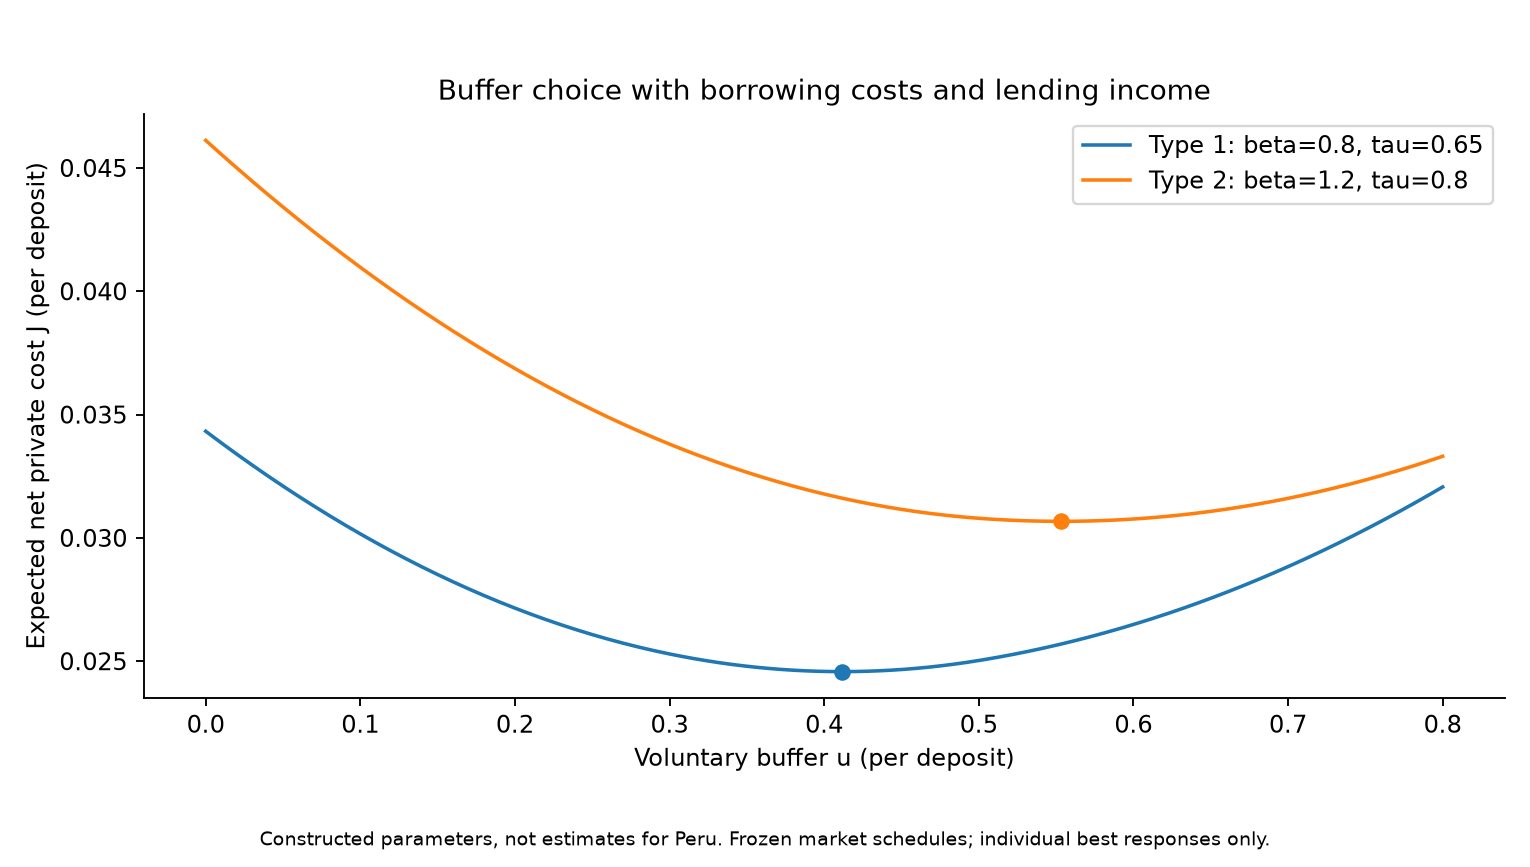
\includegraphics[width=.95\linewidth,trim=0 37 18 47,clip]
{../code/figures/post_marco/cost_and_optima.png}\par}
\vspace{-.08cm}
\figtakeaway{Type 1: $u_1^*=0.411523$ \hfill Type 2: $u_2^*=0.553381$}
\figsource{Large constructed buffers, not Peruvian estimates. Unique interiors; exposure/access differ. Truncated y-axis.}
\note{2.5 min. Source: baseline_optima.csv and cost_curves.csv.
Walk down the curve: avoided shortfalls dominate; then carrying cost dominates.
Both beta AND tau differ between types, so the level gap is not a pure access
effect. Reference buffers (0.1,0.1), NOT these choices, generated schedules.
The displayed choices are not a simultaneous equilibrium. Only redundant PNG
title/footer are cropped; inspect that axes, legend and data remain readable.}
\end{frame}

% MAIN 9.
\begin{frame}{Common capacity weakens private self-insurance}
\relax
{\small
\[
\varphi(A)=\min\{1,F/\Delta(A)\},\qquad F=\nu_F\rho D+R
\]}
\vspace{-.12cm}
\[
\boxed{\displaystyle
\frac{du_k^*}{dF}
=-\frac{\kappa\,\E_A\!\left[
1_{\{0<F<\Delta(A)\}}
\frac{(1-\psi_k)\pi_k^-}{\Delta(A)}
\right]}{J_k''(u_k^*)}\ \leq\ 0}
\]
\begin{columns}[T,onlytextwidth]
\column{.48\textwidth}
\card{Regular local optimum}{Interior; $J''>0$. Local density/IFT regularity; no coverage or uniform support kink.}
\column{.48\textwidth}
\card{Frozen environment}{$\psi_k,\ell_k,\Delta,P,Q$, prices, shock law and domain stay fixed.}
\end{columns}
\vspace{.08cm}
{\small\bfseries\color{accent}Strict $<$: a positive-probability state has
$0<F<\Delta$, $\psi_k<1$ and $\pi_k^->0$.}
\smallsource{Conditional, not general equilibrium. $F>0$; at $\Delta=0$, use $\varphi=0$.
Saturation/no exposure: weak sign only. Global stability required; full conditions in B7.}
\note{2.5 min. Phi is fixed within a u deviation but changes across F scenarios;
Delta and interbank schedules remain fixed. Strictness needs positive
probability of rationing, psi<1 and pi_minus>0 in the SAME states.
No exposure/saturation gives only a weak effect. At Delta=0 phi=0; at F=Delta
there is no asserted two-sided derivative. F=0 needs one-sided treatment.
A global best response also needs sufficiency/stability against other minima.}
\end{frame}

% MAIN 10.
\begin{frame}{More capacity, lower voluntary buffers}
\relax
{\centering
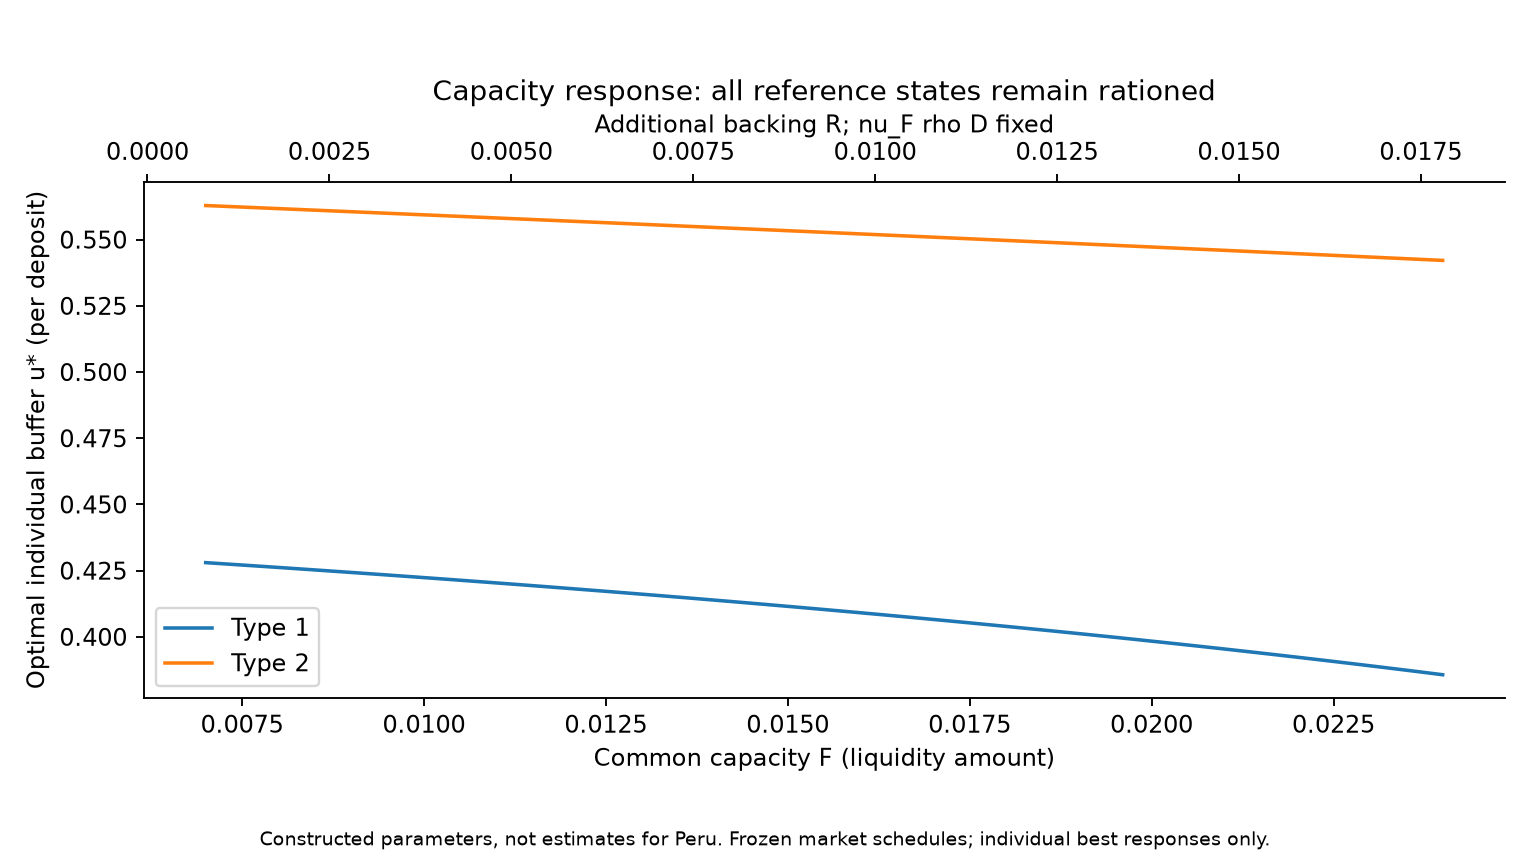
\includegraphics[width=.95\linewidth,trim=0 37 18 47,clip]
{../code/figures/post_marco/capacity_response.png}\par}
\vspace{-.08cm}
\figtakeaway{At $F=0.015$: $du_1^*/dF=-2.377540$ \hfill $du_2^*/dF=-1.214916$}
\figsource{Fixed schedules; rationed states; constructed, not GE. Truncated y-axis. Fixed-buffer $I_k$: invariant (B6).}
\note{2 min. F in [0.007,0.024], R in [0.0008,0.0178].
Reference Delta normal=0.02704, adverse=0.3843536: both remain rationed.
Slopes are per reference liquidity AMOUNT, not reserve-rate effects.
Source: capacity_sweep.csv and fixed_buffer_incidence.csv. Fixed-buffer
incidence is a separate exercise from individual u-star curves:
C_k and Cbar scale with F, which cancels from I. No directional incidence claim.}
\end{frame}

% MAIN 11.
\begin{frame}{Higher exposure raises buffers in this grid}
\relax
{\centering
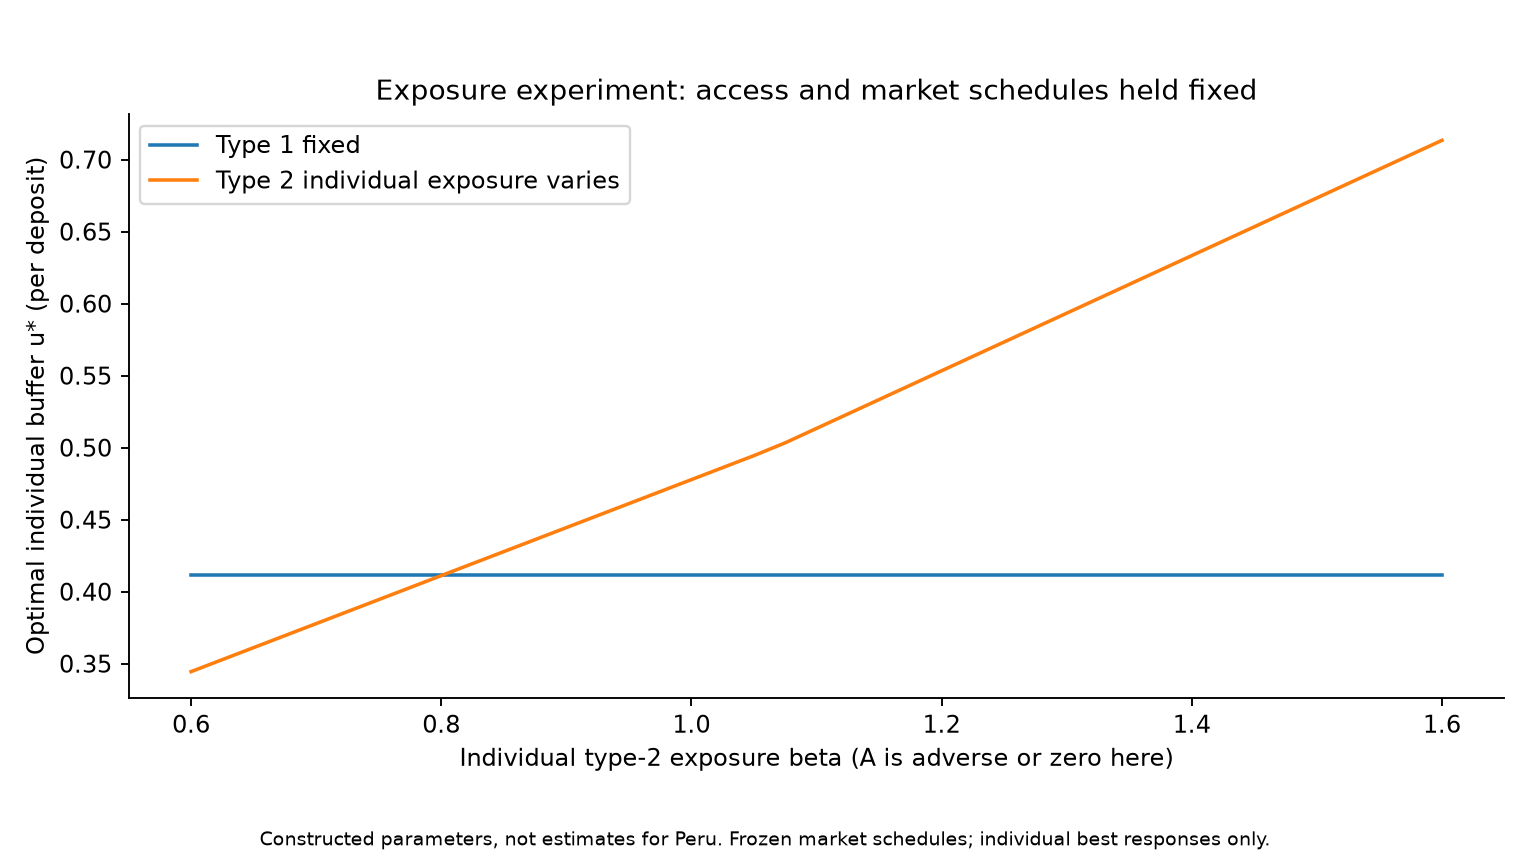
\includegraphics[width=.95\linewidth,trim=0 37 18 47,clip]
{../code/figures/post_marco/exposure_response.png}\par}
\vspace{-.08cm}
\figtakeaway{$\beta_2:0.6\to1.6$\quad $\Rightarrow$\quad $u_2^*:0.345\to0.713$\hfill Type 1 unchanged}
\figsource{One bank varies exposure; access/schedules fixed. Constructed $A\in\{-0.4,0\}$; no universal risk theorem. Truncated y-axis.}
\note{2 min. Source: exposure_sweep.csv. A single atomistic individual's beta
changes, not the entire population's exposure. For positive A, raising beta
would improve liquidity; beta is not a generic risk ordering. A slope change
near a uniform support boundary is allowed. No universal linear response
or aggregate comparative static is claimed.}
\end{frame}

% MAIN 12: authentic sources, with the original Lean type/proof excerpt.
\begin{frame}[fragile]{Two kinds of evidence, with different proof scope}
\relax
\begin{columns}[T,onlytextwidth]
\column{.53\textwidth}
\eyebrow{LEAN: AN EXISTING BUILDING BLOCK}
\[
\widehat L'(t)=-\sum_jw_j\Pi_{\sigma_j}(t-m_j).
\]
{\fontsize{8.5}{10}\selectfont
\begin{verbatim}
HasDerivAt (finiteLoss w sigma mean)
  (-finiteTail w sigma mean t) t := by

convert hd using 1
simp [finiteTail, Finset.sum_neg_distrib]
\end{verbatim}
}
{\footnotesize \texttt{finiteLoss\_derivative}: positive widths; every component off its support knots.}
\column{.42\textwidth}
\eyebrow{HUMAN: THE STUDENT'S UNIT CHECK}
\includegraphics[page=2,trim=185bp 663bp 205bp 85bp,clip,width=\linewidth]
{../hand/02-post-marco-shortfall-surplus.pdf}
{\footnotesize Authentic manuscript 02, p.~2.}\par
{\small\bfseries\color{navy}Amount: $-0.48$.\quad Ratio: $-0.30$.}\par
{\small The amount derivative carries $d_k$.}
\end{columns}
\vspace{.12cm}
\takeaway{Lean verifies supporting lemmas, not the new economic propositions.}
\smallsource{Not newly Lean-verified: the post-Marco probability/reflection bridge,
buffer FOC, capacity response or equilibrium. Genuine handwriting is a human check, not a Lean proof.}
\note{2 min. Lean excerpts remain from FiniteCompanion.lean,
finiteLoss_derivative. Reflected means m_j=-beta*A_j and t=u interpret the
new deficit; this probability/reflection bridge is not Lean-verified.
Existing package: 31 closures, no executable sorry/admit.
The crop is genuine student evidence from manuscript 02, page 2:
d_k=1.6 and pi_minus=0.3 give the amount derivative -0.48,
whereas the normalized derivative is -0.30. The manuscript records a human
verdict on this unit distinction; do not invent an earlier AI error or dispute.
All eight updated handwritten pages were reinspected independently. Manuscript
03, page 2 now uses J'(u_bar)<=0 under global convexity. Manuscript 04, page 2
establishes the local IFT branch from G=0, G_u>0 and local C1 regularity before
differentiating. Global continuation remains in the paper's full proof.
Manuscript 05 explicitly defines p_B=Pr(Delta>0) and handles zero-demand states.
Strict negative state curvature requires positive threshold density.
The existing unit-check crop remains authentic and readable; no crop change.
No new Lean proof or equilibrium result is claimed.}
\end{frame}

% MAIN 13.
\begin{frame}{A conditional answer, and three open choices}
\relax
{\fontsize{20}{24}\selectfont\bfseries\color{navy}
Common protection can reduce private buffers.\par}
{\normalsize Within the regular, frozen-schedule benchmark.}
\vspace{.25cm}
\begin{columns}[T,onlytextwidth]
\column{.315\textwidth}
\begin{beamercolorbox}[wd=\linewidth,sep=.18cm]{softbox}
{\color{accent}\Large\bfseries 01}\par
{\bfseries\color{navy}Allocation}\par
{\small Is prescribed interbank allocation an acceptable benchmark for the course/thesis transition?}
\end{beamercolorbox}
\column{.315\textwidth}
\begin{beamercolorbox}[wd=\linewidth,sep=.18cm]{softbox}
{\color{accent}\Large\bfseries 02}\par
{\bfseries\color{navy}Consistency}\par
{\small Is the conditional best response informative before solving the aggregate fixed point?}
\end{beamercolorbox}
\column{.315\textwidth}
\begin{beamercolorbox}[wd=\linewidth,sep=.18cm]{softbox}
{\color{accent}\Large\bfseries 03}\par
{\bfseries\color{navy}Next step}\par
{\small Participation incentives, shock/domain discipline, or the aggregate fixed point?}
\end{beamercolorbox}
\end{columns}
\vspace{.13cm}
\smallsource{Still open: voluntary participation; aggregate consistency; illustrative shock laws and buffer domain.
No general-equilibrium, welfare or optimal reserve-policy claim.}
\note{2 min, then invite discussion. A free fund changes outside options;
kappa>i does not establish participation. Nash cannot create trading gains
without valid outside options. No net transfers, competition, welfare or
optimal reserve-policy claim. Historical paper and Lean pin remain cf37d3f.
The course question is answered conditionally; the thesis question is open.}
\end{frame}

\appendix
\backupslidestrue
% Reference material uses a compact but consistent size; main frames stay larger.
\renewcommand{\normalsize}{\fontsize{10.5}{12.5}\selectfont}
\renewcommand{\small}{\fontsize{10}{11.6}\selectfont}
\renewcommand{\footnotesize}{\fontsize{8.5}{10}\selectfont}
\setcounter{framenumber}{0}
\begin{frame}[plain,noframenumbering]
\relax
\begin{center}
{\LARGE Backup material}\\[1em]
Accounting, constructed assumptions, proof scope and model history
\end{center}
\end{frame}

% BACKUP B1: current seven-equation benchmark, first half.
\begin{frame}{B1 \textperiodcentered{} Full benchmark: flows and allocation}
\relax
{\small All moments and schedules below are conditional on $A$.}\par\vspace{.18cm}
\begin{align}
\omega_k&=\beta_k A+\varepsilon_k,\quad s_k=d_k(\omega_k+u_k) \tag{1}\\
D_k&=\E[\pos{-s_k}\mid A],\quad X_k=\E[\pos{s_k}\mid A] \tag{2}\\
\psi_k&=\tau_k\min\{1,P/Q\},\quad \ell_k=\tau_k\min\{1,Q/P\} \tag{3}\\
\sum_k\mu_k\psi_kD_k&=\sum_k\mu_k\ell_kX_k=\min\{P,Q\}. \tag{4}
\end{align}
\[
P=\sum_k\mu_k\tau_kX_k,\quad Q=\sum_k\mu_k\tau_kD_k,\quad D=\sum_k\mu_kd_k.
\]
{\small If $P=0$ or $Q=0$, transacted volume is zero
(implemented fractions $\psi_k=\ell_k=0$).}
\smallsource{Current thesis candidate, analytical framework (1)--(4).
Prescribed quantities are not voluntary participation conditions.}
\end{frame}

% BACKUP B2.
\begin{frame}{B2 \textperiodcentered{} Full benchmark: protection and choice}
\relax
{\small
\[
\begin{aligned}
F&=\nu_F\rho D+R,\qquad \Delta=\sum_k\mu_k(1-\psi_k)D_k,\\
\varphi&=\min\{1,F/\Delta\},\quad C_k=\E_A[\varphi(1-\psi_k)D_k].
\end{aligned}\tag{5}
\]
If $\Delta=0$, set $\varphi=0$; common coverage has price $p_F=0$.
\[
\bar C=\sum_k\mu_kC_k,\qquad I_k=\frac{C_k/d_k}{\bar C/D},\quad \bar C>0. \tag{6}
\]
\[
\min_{u_k\in\mathcal U_k}
\left\{r u_k+\E_A\!\left[
i\psi_k\frac{D_k}{d_k}-i\ell_k\frac{X_k}{d_k}
+\kappa(1-\varphi)(1-\psi_k)\frac{D_k}{d_k}
\right]\right\}. \tag{7}
\]
\par\medskip
$\nu_F\in[0,1]$, $R\ge0$, $\kappa>i$.
NU reserves are not also individually usable liquidity.
$I_k$ is undefined if $\bar C=0$.}
\smallsource{Current thesis candidate (5)--(7).
Net transfers require property, repayment and loss rules not supplied here.}
\end{frame}

% BACKUP B3.
\begin{frame}{B3 \textperiodcentered{} Constructed course parameters}
\relax
\begin{columns}[T,onlytextwidth]
\column{.47\textwidth}
{\small\begin{tabular}{@{}lrr@{}}
\toprule & Type 1 & Type 2\\ \midrule
Mass $\mu_k$ & 0.6 & 0.4\\
Deposits $d_k$ & 1 & 1.6\\
Exposure $\beta_k$ & 0.8 & 1.2\\
Access $\tau_k$ & 0.65 & 0.80\\
Reference $u_k$ & 0.10 & 0.10\\
Course upper bound & 0.8 & 0.8\\ \bottomrule
\end{tabular}}
\column{.48\textwidth}
{\small\begin{tabular}{@{}lr@{}}
\toprule Common primitives & Value\\ \midrule
Carrying cost $r$ & 0.045\\
Interbank rate $i$ & 0.015\\
Uncovered cost $\kappa$ & 0.25\\
Reserve rate $\rho$ & 0.10\\
Capacity share $\nu_F$ & 0.05\\
Backing $R$ & 0.0088\\
Baseline $F$ & 0.015\\ \bottomrule
\end{tabular}}
\end{columns}
\par\medskip
{\small $A=(-0.4,0)$ with probabilities $(0.4,0.6)$;
$\varepsilon_k\mid A\sim U[-0.5,0.5]$. Aggregate deposits $D=1.24$.\\
Finite states, uniforms and $[0,0.8]$ are \textbf{course assumptions}.\\
Schedules come from reference buffers, not the displayed best responses.}
\smallsource{Source: code/output/post\_marco/parameters.json.
All parameters constructed; no Peruvian estimates or advisor approval implied.}
\end{frame}

% BACKUP B4.
\begin{frame}{B4 \textperiodcentered{} Conservation and fund feasibility}
\relax
\begin{center}
{\small\begin{tabular}{@{}lrrrr@{}}
\toprule State & $P$ & $Q$ & Borrowed = lent & Fund used\\ \midrule
Adverse & 0.0189744 & 0.2993344 & 0.0189744 & 0.015\\
Normal & 0.1623600 & 0.0721600 & 0.0721600 & 0.015\\ \bottomrule
\end{tabular}}
\end{center}
\[
\sum_k\mu_k\psi_kD_k=\min\{P,Q\}=\sum_k\mu_k\ell_kX_k,
\]
\[
\sum_k\mu_k\varphi(1-\psi_k)D_k=\min\{F,\Delta\}\le F.
\]
{\small Reference $\Delta$: adverse $0.3843536$; normal $0.02704$.\\
Checks also cover $P<Q$, $P>Q$, $P=Q$, zero sides/access,
$\Delta=0$, zero capacity and saturated coverage.}
\par\medskip
\textbf{These are reference-population accounting checks.}\\
{\small They do not make frozen-schedule best responses jointly consistent.}
\smallsource{Sources: parameters.json, reference\_market\_accounting.csv,
and verify.py: 99 checks across the three course models.}
\end{frame}

% BACKUP B5.
\begin{frame}{B5 \textperiodcentered{} Convexity, corners and a counterexample}
\relax
\[
X_k/d_k=D_k/d_k+\E[\omega_k\mid A]+u
\]
\[
J(u)=(r-\E[b_k])u+\E[(a_k-b_k)L_k]-\E[b_k\E[\omega_k\mid A]].
\]
{\small Thus $a_k\ge b_k$ gives global convexity. Otherwise this proof fails.}
\par\medskip
\textbf{Counterexample to automatic convexity:}\\
{\small Fully covered deficits give $\varphi=1$ and
$a_k-b_k=i(\psi_k-\ell_k)$.
In the adverse reference state, $\psi_1<\ell_1$.
With $F=10$, $J_1''(0.65)\simeq-0.003653$.}
\par\medskip
{\small Under convexity on $[0,\bar u]$:
\[
J'(0)\ge0\Rightarrow0\text{ minimizes},\qquad
J'(\bar u)\le0\Rightarrow\bar u\text{ minimizes}.
\]
Equalities can permit ties. The code compares every quadratic-region
endpoint/stationary point, including nonconvex and flat cases.}
\smallsource{Source: verify\_post\_marco.py; finite-uniform course specialization.}
\end{frame}

% BACKUP B6.
\begin{frame}{B6 \textperiodcentered{} Relative incidence under fixed buffers}
\relax
\[
\bar C=\sum_k\mu_kC_k,\quad I_k=\frac{C_k/d_k}{\bar C/D},\quad
\sum_k\frac{\mu_kd_k}{D}I_k=1.
\]
{\small When every state with residual deficit remains rationed and buffers
and allocation stay fixed,}
\[
C_k=F\,\E_A\!\left[\frac{(1-\psi_k)D_k}{\Delta}\right].
\]
\textbf{$F$ scales absolute coverage and cancels from relative incidence.}
\par\medskip
{\small In this constructed sweep: $I_1=1.091124$, $I_2=0.914571$;
neither changes with $F$.\\[4pt]
These are \textbf{fixed-reference-buffer} values.
Incidence with jointly reoptimized buffers needs aggregate consistency.\\[4pt]
If $\bar C=0$, $I_k$ is undefined.
Coverage shares do not identify net transfers, subsidy or welfare.}
\smallsource{Source: fixed\_buffer\_incidence.csv.
Proportional scaling does not imply directional heterogeneous incidence.}
\end{frame}

% BACKUP B7.
\begin{frame}{B7 \textperiodcentered{} Exact conditions for the capacity result}
\relax
{\small\begin{enumerate}
\item Fixed deposits, domain, shock law, $r,i,\kappa$;
fixed $\psi_k,\ell_k,\Delta,P,Q$. Only $\varphi$ changes with $F$.
\item Regular differentiable interior optimum branch, $J''(u^*)>0$;
no competing global-minimum switch.
\item Valid derivative/expectation interchange. Finite-state uniforms:
positive widths and no relevant support knot.
\item $F>0$, no relevant $F=\Delta(A)$ kink.
If $\Delta=0$, use the stated zero-coverage convention.
\item Strict negativity requires positive-probability states with
$F<\Delta$, $\psi_k<1$, and $\pi_k^->0$.
Otherwise only a weak sign is justified.
\end{enumerate}
\par\medskip
The implicit-function argument gives a \textbf{local} response.
Global best-response language needs global sufficiency/stability.\\[4pt]
Holding $\nu_F,\rho,D$ fixed gives $du^*/dR=du^*/dF$.
It does not give a reserve-rate, GE or participation theorem.}
\smallsource{POST\_MARCO\_AUDIT.md, section 4.
Corners, ties, saturation and one-sided boundary questions are separate.}
\end{frame}

% BACKUP B8.
\begin{frame}{B8 \textperiodcentered{} What changed across the course}
\relax
{\small\begin{tabular}{@{}>{\raggedright\arraybackslash}p{.18\linewidth}>{\raggedright\arraybackslash}p{.23\linewidth}>{\raggedright\arraybackslash}p{.24\linewidth}>{\raggedright\arraybackslash}p{.25\linewidth}@{}}
\toprule & October & November 4 & Current post-Marco\\ \midrule
Core & Two currencies; public dollar backing & Direct support; asset-linked eligibility &
One USD currency; prescribed interbank allocation\\[7pt]
Buffer benefit & Avoid deficit costs & Avoid financing and deferral costs &
Avoid deficit costs AND earn lending income\\[7pt]
$\varphi$ meaning & Common/public coverage & Reserve usability & Common coverage fraction\\[7pt]
Comparative static & Conditional backing effect & Conditional reserve-burden effect &
Conditional capacity effect\\ \bottomrule
\end{tabular}}
\par\medskip
\textbf{Historical work is preserved; its equations are not silently reused.}\\
{\small Existing Lean package remains pinned to paper \texttt{cf37d3f}.
Current economic source: accepted post-Marco computational checkpoint.}
\end{frame}

% BACKUP B9. Existing theorem with line wrapping only.
\begin{frame}[fragile]{B9 \textperiodcentered{} Existing Lean proof and scope}
\relax
{\footnotesize \texttt{Gomez26EligibilityBuffers.ell\_derivative}
(\texttt{BufferCore.lean}), unchanged:}
{\fontsize{8.8}{10.2}\selectfont
\begin{verbatim}
theorem ell_derivative {sigma z : ℝ} (hs : 0 < sigma)
    (hnl : z ≠ -sigma) (hnu : z ≠ sigma) :
    HasDerivAt (ell sigma) (-piTail sigma z) z := by
  by_cases hl : z ≤ -sigma
  · simpa [piTail, hl] using ell_derivative_below
      (lt_of_le_of_ne hl hnl)
  · by_cases hu : z < sigma
    · simp only [piTail, if_neg hl, if_pos hu]
      convert ell_derivative_inside hs
        (lt_of_not_ge hl) hu using 1; ring
    · simpa [piTail, hl, hu] using
        ell_derivative_above hs
          (lt_of_le_of_ne (le_of_not_gt hu) hnu.symm)
\end{verbatim}
}
{\small New deficit input: $z=u+\beta A$
(equivalently finite-loss means $m_j=-\beta A_j$).\\
Reflecting the symmetric uniform shock gives the probability interpretation;
that bridge and the new economic propositions are not already Lean proofs.}
\note{Source: exact existing ell_derivative body, line wrapping only.
It proves the explicit function derivative off both support knots.
The finiteLoss theorem sums/chains this result. There are 31 old closures,
not a newly formalized post-Marco FOC, capacity theorem or equilibrium.}
\end{frame}
\end{document}
